\documentclass{article}
\usepackage{amsmath}
%\usepackage{psfig}

\usepackage{amsmath}
\usepackage{graphicx}
\usepackage{float}
\usepackage{amssymb} 
\usepackage{amsthm}
\usepackage{pgf}
\usepackage{tikz}
\usetikzlibrary{automata,shapes.multipart} %
\usetikzlibrary{arrows,petri}
\usepackage[latin1]{inputenc}
%\usepackage[noend]{algorithmic}
\usepackage{algorithm}
%\usepackage{algo}
\usepackage{epsfig}
\usepackage{subfigure}
\usepackage{multirow}
\usepackage{url}

\newcommand{\cosmos}{\mbox{\textup{C}\scalebox{0.75}{{\textsc{OSMOS}}}}}
\newcommand{\cosyverif}{\mbox{\textup{C}\scalebox{0.75}{{\textsc{OSY}}}\textup{V}\scalebox{0.75}{{\textsc{ERIF}}}}}

\title{\cosmos{} User Manual}
\author{Beno\^it Barbot}

\begin{document}
\maketitle


This is the user manual for the tool \cosmos{} version 1.4

\section{Tool Usage}

\subsection{Basic Usage}
The primary usage of the tool \cosmos{} is as follow:
\begin{verbatim}
Cosmos model property
\end{verbatim}
where the model is specified in the GRML file format or in the
\verb|.grml| file format and the property is expressed either in GRML
or in the \verb|.lha| file format.

\subsubsection{Model}
Models taken by \cosmos{} as input are variant of Petri net.  The main
model supported by \cosmos are Stochastic Petri net with inhibitor
arcs and general distribution. The file format of \cosyverif{} (GRML) 
allows to specified different variant of Petri Net which are also 
recognize by \cosmos{}:
\begin{itemize}
\item Plain Petri net can be read in this case exponential distribution of 
  rate $1$ is assign to each transition.
\item Stochastic Petri net with inhibitor arc and general distribution.
\item Symmetric Net, like for plain Petri net in this case exponential
  distribution of rate $1$ are assume.
\item Stochastic Symmetric Net. 
\end{itemize}
The specification of file format are reported in Section{sec:fileformat}.

\subsubsection{Property}
Property are specified in the Hybrid Linear Automaton Logic(HASL)
which as the name suggest relies on Linear Hybrid Automaton(LHA) to
select path and on several HASL expression to specify various
performance values.

\subsection{Statistical Options}
Several options can be used to control the behaviors of the statistical engine.
The default behaviors is to simulate trajectories until either
\begin{itemize}
\item The maximum number of trajectories is reach.
\item The specified width for confidence intervals is reach.
\end{itemize}

\subsubsection{\texttt{--width arg}  option}
This option specified \texttt{arg} as the objective width for
confidence intervals. If it is set to $0$ trajectories are
simulated until the maximum number of trajectories is reached.
The default value is $0.001$.

\subsubsection{\texttt{--max-run arg}  option}
This option specified \texttt{arg} as the maximal number of run.
The default value is $2,000,000$.

\subsubsection{\texttt{--level arg}  option}
This option set the confidence level to \texttt{arg}.
The default value is $0.99$.

\subsubsection{\texttt{--batch arg}  option}
This option set the number of simulation to perform between each
statistical test.  The default value is $1000$. When this value is 
set to $0$ the tool will perform a test at constant time period.

\subsubsection{\texttt{--njob arg}  option}
This option set the number of parallel computation to \texttt{arg}.
The default value is $1$.

\subsubsection{\texttt{--relative}  option}
This option set allow cosmos to used relative confidence interval
instead of absolute one.

\subsubsection{\texttt{--chernoff arg}  option}
This option use chernoff-hoeffding bound to compute statistical parameter.
\texttt{arg} contain one of \texttt{width,level,nbrun}. The parameter 
specified by \texttt{arg} is computed using Chernoff-Hoeffding bound.

\subsection{Input Options}

\subsubsection{\texttt{--const X1=c1,X2=c2,\dots,Xn=cn}  option}
This option overrides values of constants of models. The constants is
define if it was done define in the model before.

\subsubsection{\texttt{-g, --grml-input}  option}
This option force the tool to use the GRML parser for the model and
the LHA. This is mostly deprecated as the correct parser is inferred
from the extension.

\subsubsection{\texttt{--HASL-expression arg}  option}
This allow to specify additional HASL{} expressions to the automaton.
The syntax of \texttt{arg} is the one of HASL{} expression in the
\texttt{.lha} file format and should ends with ``\texttt{;}''.

\subsubsection{\texttt{--loop arg [--transient arg2]}  option}
This produce a set of HASL formulas evaluating the mean number of 
token in each place and the mean throughput of each transition until time
\texttt{arg}. The optional additional argument allows to specify a transient
time where the mean number of token and throughput are not recorded.
See option \texttt{--trace-place} to specify which places and transitions 
to monitor.

\subsubsection{\texttt{--sampling t1 t2} option}
This produce an automaton that sample each \texttt{t2} time unit the
mean number of token in each place for this period, until time
\texttt{t1} is reached.  See option \texttt{--output-graph} to format
the output in a more manageable way.

\subsubsection{\texttt{--count-transition} option}
This Produce a set of HASL formulas counting the number of firing of each
transition.

\subsubsection{\texttt{--formula arg} option}
Send the expression \texttt{arg} to the \emph{AutomataGen} tool to produce
the LHA used for the simulation. The tool AutomataGen is a work in progress.

\subsection{Output formatting Options}
The default behavior of \cosmos{} for displaying result is as follows:
During the simulation a synthetic overview is displayed:
\begin{scriptsize}
\begin{verbatim}
Total paths: 28570000  Accepted paths: 22442000  Wall-clock time: 21s  Remaining(approx): 32s  Trajectory per second: 1.4e+06
r:        |< 2.639128431e-08 --[ 0.4999066088    < 0.5000635601    > 0.5002205154    ]-- 0.9999999687    >| width=0.000313902
pi:       |< 0               --[ 3.141245613     < 3.142037101     > 3.142828210     ]-- 4               >| width=0.001582596
pi2:      |< 0               --[ 0.7853114033    < 0.7855092754    > 0.7857070525    ]-- 1               >| width=0.000395649
% of Err: [||||||||||||||||||||||||||||||||||||||||                                                       ] 39%	
% of run: [||||||||||||||||||||||||||||                                                                   ] 28%	
\end{verbatim}
\end{scriptsize}
The first line provide information on the speed of simulation. The
remaining time is computed assuming that the size of confidence
interval decrease in $1/\sqrt{N}$ with $N$ the number of trajectories.
The second to fourth line present three HASL expressions. The first
number is minimal value observed for this expression, then the lower
bound of the confidence interval is displayed, then the estimated
value, then the upper bound and then the maximal observed value. The
width of the confidence interval is displayed at the end.  The last
two lines show progress bar indicating the progress of the
simulation. The first one indicate the progress to reach specified
confidence interval width limit. This progress is corrected assuming
that the width progress in $1/\sqrt{N}$ thus this bar progress at
constant speed. The last bar is the number of simulated trajectory 
compare to the maximal number of trajectories.

When the simulation finished results are return in key-value format
easier to parse for tools:
\begin{scriptsize}
\begin{verbatim}
Model path:	pi.gspn
LHA path:	pi.lha
r:
Estimated value:	0.500031454383448
Confidence interval:	[0.499932270760877 , 0.50013063800602]
Minimal and maximal value:	[1.93365088646926e-08 , 0.999999971987635]
Width:	0.000198367245143327
pi:
Estimated value:	3.14176752504576
Confidence interval:	[3.14126745104347 , 3.1422674472686]
Minimal and maximal value:	[0 , 4]
Width:	0.000999996225129696
pi2:
Estimated value:	0.78544188126144
Confidence interval:	[0.785316862760866 , 0.785566861817149]
Minimal and maximal value:	[0 , 1]
Width:	0.000249999056282424
Method:	Confidence interval computed sequentially using Chows-Robbin algorithm or SPRT.
Confidence level:	0.99
Total paths:	71569000
Accepted paths:	56213290
Batch size:	1000
Time for simulation:	55.245259s
Total CPU time:	60.068667
Total Memory used:	44.87 MB
Number of jobs:	1
Results are saved in 'Result_pi.res'
Results are saved in 'Result.res'
\end{verbatim}
\end{scriptsize}
All the simulations parameters are recalled. The additional
information are the \texttt{Time for simulation} which is the wall
clock time uses by the simulation.  It decrease when the number of
parallel processes increases on multi-processor machine.  The
\texttt{Total CPU time} is the cpu time consume by the whole
computation it slightly increases when the number of parallel process
increases. The \texttt{Total Memory used} line report the memory used
by the whole computation. In most cases the maximum memory consumption
is reached during the compilation of the simulator and highly depends of
the compiler used. This output is also stored in a file called \texttt{Result.res}.

Several option allow to output other data from the simulation:

\subsubsection{\texttt{-v, --verbose arg} option}
Set the verbose level of the tool. The default is $2$, with $0$ the tool
does not write anything on the standard output. The maximum is $6$ which 
generate debug information at each step of the simulation.

\subsubsection{\texttt{-i,--interactive} option}
This option allows to debug a model by stopping the simulation after
each step.  This is option should not be used together with
\texttt{--njob n} with $n>1$.  When the simulation is stopped the user
is asked either to type \texttt{step} to fire the following transition
or \texttt{fire tr} where \texttt{tr} is the name of an enabled
transition. This mode is not fully compatible with stochastic
symmetric net as the command \texttt{fire} does not allows to specify
a binding.

\subsubsection{\texttt{--output-graph arg} option}
Allows to output results of HASL formula in a blank separated file
format. The argument \texttt{arg} specify the name of the file.  This
is well suited for HASL expressions specifying a graph like
\texttt{PDF, CDF} or the expression generated by the
\texttt{--sampling} option.  Figure~\ref{fig:sampling} show a graph
generated by the \texttt{--sampling 2 0.001} option on the shared
memory example. The \texttt{--output-graph} option generate a file
starting as file:
\begin{scriptsize}
\begin{verbatim}
abscissa MeanToken_Access1_low MeanToken_Access1_mean MeanToken_Access1_up           ... 
0.005 7.6218e-05 0.000144057 0.000211896 0.00920415 0.00986402 0.0105239 0.000103712 ...
0.015 0.000803674 0.00103768 0.00127168 0.0279092 0.0292027 0.0304962 0.000759281    ...
...
\end{verbatim}
\end{scriptsize}
which can easily be plotted as the figure using \texttt{gnuplot}.
This can be used for user defined HASL formula by using name ending by
\verb|$GRAPH$x1$x2$| for HASL expressions where $(x1+x2)/2$ is the
abcsissa of the point computed by the expression.

\begin{figure}[h]
  \centering
  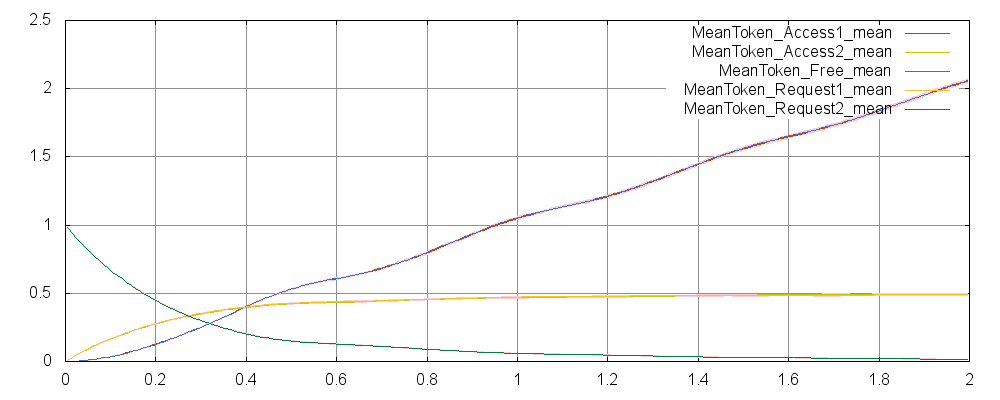
\includegraphics[width=1.01\textwidth]{figures/sampling.png}
  \caption{Sampling the trajectories of the shared memory example}
  \label{fig:sampling}
\end{figure}

\subsubsection{\texttt{-d, --output-data arg} option}
This option generate a file 


\section{File Format}
\label{sec:fileformat}
\subsection{Generalized Stochastic Petri Net (.gspn)}
This file format is used to describe GSPN.
First we describe an example:\\
\begin{figure}[h]
  \centering
  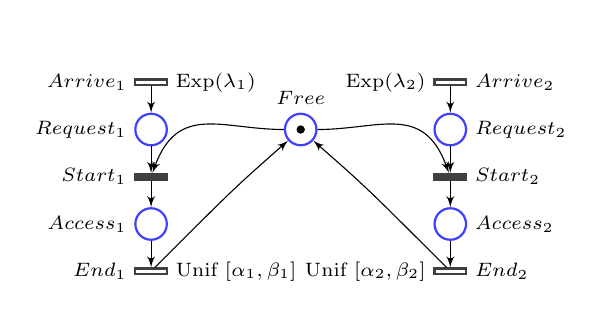
\begin{tikzpicture}[node distance=0.6cm,>=stealth',auto]
{\scriptsize
  \tikzstyle{place}=[circle,thick,draw=blue!75,minimum size=4mm]
  \tikzstyle{transition}=[rectangle,thick,draw=black!75,
  minimum width=4mm,inner sep=0pt,minimum height=.7mm]

    \node [] (i1)       {};
    \node [transition,label=left:$Arrive_1$,label=right:Exp($\lambda_1$)] (tr1) [below of =i1]{};
    \node [place,label=left:$Request_1$] (r1) [below of=tr1]  {};
    \node [transition,,label=left:$Start_1$,fill=black!75] (ta1) [below of =r1]{}; %label=right:$(\mbox{pri}_1\colon w_1)$
    \node [place,label=left:$Access_1$] (a1)  [below of=ta1] {};
    \node [transition,label=left:$End_1$,label=right:{\hspace{-0mm}{\scriptsize Unif $[\alpha_1,\beta_1]$}}] (ti1) [below of =a1]{};
    \node [place,tokens=1,label=above:$Free$] (f) [right of=r1,xshift=13mm]    {};
    \node [place,label=right:$Request_2$] (r2) [right of=f,xshift=13mm]    {};
   \node [transition,label=right:$Arrive_2$,label=left:Exp($\lambda_2$)] (tr2) [above of =r2]{};
    \node [] (i2) [above of=tr2]    {};
    \node [transition,label=right:$Start_2$,fill=black!75] (ta2) [below of =r2]{}; %label=left:$(\mbox{pri}_2\colon w_2)$,
    \node [place,label=right:$Access_2$] (a2) [below of=ta2]    {};
    \node [transition,label=right:$End_2$,label=left:{\hspace{-2mm}{\scriptsize Unif $[\alpha_2,\beta_2]$}}] (ti2) [below of =a2]{};
%\draw [-latex'] (i1) to (tr1);
\draw [-latex'] (tr1) to (r1);
\draw [-latex'] (r1) to (ta1);
\draw [-latex'] (ta1) to (a1);
\draw [-latex'] (a1) to (ti1);
%\draw [-latex'] (i2) to (tr2);
\draw [-latex'] (tr2) to (r2);
\draw [-latex'] (r2) to (ta2);
\draw [-latex'] (ta2) to (a2);
\draw [-latex'] (a2) to (ti2);
\draw [-latex'] (f) .. controls +(0:10mm) and +(110:10mm) .. (ta2);
\draw [-latex'] (f) .. controls +(180:10mm) and +(70:10mm) .. (ta1);
\draw [-latex'] (ti1) .. controls +(45:15mm)  .. (f); %and +(260:20mm)
\draw [-latex'] (ti2) .. controls +(135:15mm) .. (f); %and +(280:20mm) 
}
\end{tikzpicture} 
  \caption{Infinite-state GSPN  model of a shared memory system.}
  \label{fig:sharedmem}
  % \vspace*{-.3cm}
\end{figure}
This GSPN is described by the following text:
\begin{verbatim}
const double lambda1 = 1;
const double lambda2 = 2;
const double alpha1 = 1;
const double alpha2 = 1;
const double beta1 = 5;
const double beta2 = 5;

NbPlaces = 5;
NbTransitions = 6;

PlacesList = { 
   Request_1, Request_2,
   Access_1, Access_2,
   Free
} ;

TransitionsList = { 
   Arrive_1,Arrive_2,
   Start_1 ,Start_2,
   End_1   ,End_2
} ;

Marking={
   (Request_1 , 0); (Request_2 , 0) ; 
   (Access_1 , 0) ; (Access_2 , 0) ;
   (Free, 1);
};

Transitions={
   (Arrive_1,EXPONENTIAL(lambda1),1,1, SINGLE); 
   (Arrive_2,EXPONENTIAL(lambda2),1,1, SINGLE);
   (Start_1,DETERMINISTIC(0),1,1); 
   (Start_2,DETERMINISTIC(0),1,1);
   (End_1,UNIFORM(alpha1,beta1),1,1); 
   (End_2,UNIFORM(alpha2,beta2),1,1);
};

InArcs={
   (Request_1,Start_1,1); (Free,Start_1,1);
   (Request_2,Start_2,1); (Free,Start_2,1);
   (Access_1,End_1,1);
   (Access_2,End_2,1);
};

OutArcs={
   (Arrive_1,Request_1,1); 
   (Arrive_2,Request_2,1);
   (End_1,Free,1);
   (End_2,Free,1);
};
\end{verbatim}

{\bf Description:}
The first bloc is a list of constants definition, constants can be
either \verb|double| or \verb|int|.\\
Then we specify the number of place and transitions with:
\verb|NbPlaces = 5; NbTransitions = 6;|\\
The list of place name and transition name is given in the
\verb|PlacesList| and \verb|TransitionsList| statement.\\
The initial marking of the net is given as a set of pairs
in the \verb|Marking| statement.\\
The transition distribution is given as a set of tuples like
this one:\\ \verb|(Arrive_1,EXPONENTIAL(lambda1),1,1, SINGLE)|
each tuple contain first the name of the transition then
the probability distribution with some parameters, then two positive
reals define the priority and weight of the event generated.
For exponential distribution we can specify the policy of service
which can be \verb|SINGLE,INFINITE,MULTIPLE(n)|.\\
Finally come the description of arcs of the net with the 
\verb|InArcs|,\verb|OutArcs| and \verb|InhibitorsArcs| statements.



\subsubsection{Grammar}
the complete grammar is:
\begin{verbatim}
$accept: GSPN "end of file"

GSPN: declarations definitions
    | declarations definitions redifinitions

declarations: Constants Sizes Lists
            | Sizes Lists

Constants: Constant
         | Constant Constants

Constant: 'const' 'int' str '=' IntStringFormula ';'
        | 'const' 'double' str '=' RealStringFormula ';'

IntStringFormula: ival
                | str
                | '(' IntStringFormula ')'
                | IntStringFormula '+' IntStringFormula
                | IntStringFormula '-' IntStringFormula
                | IntStringFormula '*' IntStringFormula
                | IntStringFormula '^' IntStringFormula
                | FLOOR '(' IntStringFormula ')'
                | FLOOR '(' IntStringFormula '/' IntStringFormula ')'
                | MIN '(' IntStringFormula ',' IntStringFormula ')'
                | MAX '(' IntStringFormula ',' IntStringFormula ')'

RealStringFormula: rval
                 | ival
                 | str
                 | '(' RealStringFormula ')'
                 | RealStringFormula '/' RealStringFormula
                 | RealStringFormula '+' RealStringFormula
                 | RealStringFormula '-' RealStringFormula
                 | RealStringFormula '*' RealStringFormula
                 | RealStringFormula '^' RealStringFormula
                 | FLOOR '(' RealStringFormula ')'
                 | MIN '(' RealStringFormula ',' RealStringFormula ')'
                 | MAX '(' RealStringFormula ',' RealStringFormula ')'

Sizes: NbPlaces NbTransitions
     | NbTransitions NbPlaces

NbPlaces: 'NbPlaces' '=' ival ';'
        | 'NbPlaces' '=' str ';'

NbTransitions: 'NbTransitions' '=' ival ';'
             | 'NbTransitions' '=' str ';'

Lists: PlacesList TransitionsList
     | TransitionsList PlacesList

PlacesList: 'PlacesList' '=' '{' PLabels '}' ';'

PLabels: str
       | PLabels ',' str

TransitionsList: 'TransitionList' '=' '{' TLabels '}' ';'

TLabels: str
       | TLabels ',' str

definitions: PlacesDef TransitionsDef InArcs OutArcs
           | PlacesDef TransitionsDef InArcs OutArcs Inhibitors

PlacesDef: 'Marking' '=' '{' PLACES '}' ';'

PLACES: PLACE
      | PLACES PLACE

PLACE: '(' str ',' IntStringFormula ')' ';'

TransitionsDef: 'Transition' '=' '{' TRANSITIONS '}' ';'

TRANSITIONS: TRANSITION
           | TRANSITIONS TRANSITION

TRANSITION: '(' str ',' dist ',' PRIORITY ',' WEIGHT ')' ';'
          | '(' str ',' 'EXPONENTIAL' '(' RealStringFormula ')' ',' PRIORITY ',' 
            WEIGHT ',' SERVICE ')' ';'
          | '(' str ',' IMDT ',' PRIORITY ',' WEIGHT ')' ';'

dist: str '(' params ')'

params: RealStringFormula
      | params ',' RealStringFormula

WEIGHT: RealStringFormula

PRIORITY: RealStringFormula

SERVICE: 'SINGLE'
       | 'INFINITE'
       | 'MULTIPLE' '(' ival ')'
       | 'MULTIPLE' '(' str ')'

InArcs: 'InArcs' '=' '{' incells '}' ';'

incells: incell
       | incells incell

incell: '(' str ',' str ',' IntStringFormula ')' ';'
      | '(' str ',' str ')' ';'

OutArcs: 'OutArcs' '=' '{' outcells '}' ';'

outcells: outcell
        | outcells outcell

outcell: '(' str ',' str ',' IntStringFormula ')' ';'
       | '(' str ',' str ')' ';'

Inhibitors: 'inhibitor' '=' '{' inhibcells '}' ';'

inhibcells: inhibcell
          | inhibcells inhibcell

inhibcell: '(' str ',' str ',' IntStringFormula ')' ';'
         | '(' str ',' str ')' ';'
\end{verbatim}




\end{document}
